\documentclass[a4paper, 12pt, openany]{book}

%%% Работа с русским языком % для pdfLatex
\usepackage{cmap}					% поиск в~PDF
\usepackage{mathtext} 				% русские буквы в~фомулах
\usepackage[T2A]{fontenc}			% кодировка
\usepackage[utf8]{inputenc}			% кодировка исходного текста
\usepackage[english,russian]{babel}	% локализация и переносы
\usepackage{indentfirst} 			% отступ 1 абзаца
\usepackage{gensymb}				% мат символы?

%%% Работа с русским языком % для XeLatex
%\usepackage[english,russian]{babel}   %% загружает пакет многоязыковой вёрстки
%\usepackage{fontspec}      %% подготавливает загрузку шрифтов Open Type, True Type и др.
%\defaultfontfeatures{Ligatures={TeX},Renderer=Basic}  %% свойства шрифтов по умолчанию
%\setmainfont[Ligatures={TeX,Historic}]{Times New Roman} %% задаёт основной шрифт документа
%\setsansfont{Comic Sans MS}                    %% задаёт шрифт без засечек
%\setmonofont{Courier New}
%\usepackage{indentfirst}
%\frenchspacing

%%% Дополнительная работа с математикой
\usepackage{amsfonts,amssymb,amsthm,mathtools}
\usepackage{amsmath}
\usepackage{icomma} % "Умная" запятая: $0,2$ --- число, $0, 2$ --- перечисление
\usepackage{upgreek}

%% Номера формул
%\mathtoolsset{showonlyrefs=true} % Показывать номера только у тех формул, на которые есть \eqref{} в~тексте.

%%% Страница
\usepackage{extsizes} % Возможность сделать 14-й шрифт

%% Шрифты
\usepackage{euscript}	 % Шрифт Евклид
\usepackage{mathrsfs} % Красивый матшрифт

%% Свои команды
\DeclareMathOperator{\sgn}{\mathop{sgn}} % создание новой конанды \sgn (типо как \sin)
\DeclareMathOperator{\rg}{\mathop{rg}}
\DeclareMathOperator{\Rg}{\mathop{Rg}}
\DeclareMathOperator{\im}{\mathop{Im}}
\DeclareMathOperator{\tr}{\mathop{tr}}
\DeclareMathOperator{\const}{\mathop{const}}
\DeclareMathOperator{\Id}{\mathop{Id}}
%\DeclareMathOperator{\dim}{\mathop{dim}}
\usepackage{csquotes} % ещё одна штука для цитат
\newcommand{\pd}[2]{\ensuremath{\cfrac{\partial #1}{\partial #2}}} % частная производная
\newcommand{\abs}[1]{\ensuremath{\left|#1\right|}} % модуль
\renewcommand{\phi}{\ensuremath{\varphi}} % греческая фи
\newcommand{\pogk}[1]{\!\left(\cfrac{\sigma_{#1}}{#1}\right)^{\!\!\!2}\!} % для погрешностей


%\renewcommand{\labelenumi}{\asbuk{enumi})}

% Ссылки
\usepackage{color} % подключить пакет color
% выбрать цвета
\definecolor{BlueGreen}{RGB}{49,152,255}
\definecolor{Violet}{RGB}{120,80,120}
% назначить цвета при подключении hyperref
\usepackage[unicode, colorlinks, urlcolor=blue, linkcolor=blue, pagecolor=blue, citecolor=blue]{hyperref} %синие ссылки
%\usepackage[unicode, colorlinks, urlcolor=black, linkcolor=black, pagecolor=black, citecolor=black]{hyperref} % для печати (отключить верхний!)


%% Перенос знаков в~формулах (по Львовскому)
\newcommand*{\hm}[1]{#1\nobreak\discretionary{}
	{\hbox{$\mathsurround=0pt #1$}}{}}

%%% Работа с картинками
\usepackage{graphicx}  % Для вставки рисунков
\graphicspath{{images/}{images2/}}  % папки с картинками
\setlength\fboxsep{3pt} % Отступ рамки \fbox{} от рисунка
\setlength\fboxrule{1pt} % Толщина линий рамки \fbox{}
\usepackage{wrapfig} % Обтекание рисунков и таблиц текстом
\usepackage{multicol}

%%% Работа с таблицами
\usepackage{array,tabularx,tabulary,booktabs} % Дополнительная работа с таблицами
\usepackage{longtable}  % Длинные таблицы
\usepackage{multirow} % Слияние строк в~таблице
\usepackage{caption}
\captionsetup{labelsep=period, labelfont=bf}

%%% Оформление
\usepackage{indentfirst} % Красная строка
%\setlength{\parskip}{0.3cm} % отступы между абзацами
%%% Название разделов
\usepackage{titlesec}
\titlelabel{\thetitle.\quad}
\renewcommand{\figurename}{\textbf{Рис.}}		%Чтобы вместо figure под рисунками писал "рис"
\renewcommand{\tablename}{\textbf{Таблица}}		%Чтобы вместо table над таблицами писал Таблица
\usepackage{enumitem}
\setlist{nolistsep}
\usepackage{verbatim}

%%% Теоремы
\theoremstyle{plain} % Это стиль по умолчанию, его можно не переопределять.
\newtheorem{theorem}{Теорема}[section]
\newtheorem{proposition}[theorem]{Утверждение}
\newtheorem{predlog}{Предложение}[section]
\newtheorem{lemma}{Лемма}[section]

\theoremstyle{definition} % "Определение"
\newtheorem{definition}{Определение}[section]
\newtheorem{corollary}{Следствие}[theorem]
\newtheorem{problem}{Задача}[section]

\theoremstyle{remark} % "Примечание"
\newtheorem*{nonum}{Решение}
\newtheorem{zamech}{Замечание}[theorem]

%%% Правильные мат. символы для русского языка
\renewcommand{\epsilon}{\ensuremath{\varepsilon}}
\renewcommand{\phi}{\ensuremath{\varphi}}
\renewcommand{\kappa}{\ensuremath{\varkappa}}
\renewcommand{\le}{\ensuremath{\leqslant}}
\renewcommand{\leq}{\ensuremath{\leqslant}}
\renewcommand{\ge}{\ensuremath{\geqslant}}
\renewcommand{\geq}{\ensuremath{\geqslant}}
\renewcommand{\emptyset}{\varnothing}

%%% Для лекций по инфе
\usepackage{alltt}
\newcounter{infa}[section]
\newcounter{num}
\definecolor{infa}{rgb}{0, 0.2, 0.89}
\definecolor{infa1}{rgb}{0, 0.3, 1}
\definecolor{grey}{rgb}{0.5, 0.5, 0.5}
\newcommand{\tab}{\ \ \ }
\newcommand{\com}[1]{{\color{grey}\##1}}
\newcommand{\num}{\addtocounter{num}{1}\arabic{num}\tab}
\newcommand{\defi}{{\color{infa}def}}
\newcommand{\ini}{{\color{infa}in}}
\newcommand{\rangei}{{\color{infa}range}}
\newcommand{\fori}{{\color{infa}for}}
\newcommand{\ifi}{{\color{infa}if}}
\newcommand{\elsei}{{\color{infa}else}}
\newcommand{\printi}{{\color{infa1}print}}
\newcommand{\maxi}{{\color{infa}max}}
\newcommand{\classi}{{\color{infa}class}}
\newcommand{\returni}{{\color{infa}return}}
\newcommand{\elifi}{{\color{infa}elif}}


\newenvironment{infa}[1]{
	
	\vspace{0.5cm}
	\addtocounter{infa}{1}%
	\noindent{\large \textbf{Программа №\thesection.\arabic{infa}}}\textbf{<<#1>>}%
	\begin{alltt}%
	}{\end{alltt}
	\setcounter{num}{0}
	\vspace{0.1cm}}
%Пример кода:
%\begin{infa}{Поразрядная сортировка}
%	\ \num \defi count_sort(a):\tab \com{определяет нашу функцию}
%	\ \num \tab m = \maxi(a)+1
%	\ \num \tab q = [0]*m
%	\ \num \tab \fori x \ini a:
%	\ \num \tab \tab q[x] += 1
%	\ \num \tab pos = 0
%	\ \num \tab \fori x \ini q:
%	\ \num \tab \tab \fori i \ini \rangei(q[x]):
%	\ \num \tab \tab \tab a[pos] = x
%	\num \tab \tab \tab pos += 1
%\end{infa}

\usepackage{titlesec}
\titlelabel{\thetitle.\quad}

\usepackage{biblatex}
\addbibresource{references.bib}

\usepackage[left=1.27cm,right=1.27cm,top=2cm,bottom=2cm]{geometry}

\usepackage{fancyhdr} % Для колонтитулов

\renewcommand{\baselinestretch}{1.3}

\makeatletter % Убирает нумерацию на страницах, где \chapter
\renewcommand\chapter{\if@openright\cleardoublepage\else\clearpage\fi
	\thispagestyle{empty}% original style: plain
	\global\@topnum\z@
	\@afterindentfalse
	\secdef\@chapter\@schapter}
\makeatother

\usepackage{fancyhdr}
\pagestyle{fancy}
\fancyhf{}
\fancyhead[L]{\rightmark}
\fancyhead[R]{\textbf{\thepage}}

\setcounter{secnumdepth}{0}

\newcommand\invisiblesection[1]{%
	\refstepcounter{section}%
	\addcontentsline{toc}{section}{#1}%
	\sectionmark{#1}}


\title{Вопрос по выбору}
\author{Алексей Кожарин}
\date{\today}
\usepackage[left=1.27cm,right=1.27cm,top=2cm,bottom=2cm]{geometry}

\usepackage{fancyhdr} % Для колонтитулов

\renewcommand{\baselinestretch}{1.3}

\makeatletter % Убирает нумерацию на страницах, где \chapter
\renewcommand\chapter{\if@openright\cleardoublepage\else\clearpage\fi
	\thispagestyle{empty}% original style: plain
	\global\@topnum\z@
	\@afterindentfalse
	\secdef\@chapter\@schapter}
\makeatother

\usepackage{fancyhdr}
\pagestyle{fancy}
\fancyhf{}
\fancyhead[L]{\rightmark}
\fancyhead[R]{\textbf{\thepage}}

\setcounter{secnumdepth}{0}

\newcommand\invisiblesection[1]{%
	\refstepcounter{section}%
	\addcontentsline{toc}{section}{#1}%
	\sectionmark{#1}}


\begin{document}
	\begin{titlepage}
\begin{center} 
 
\large Московский физико-технический институт\\
Факультет молекулярной и химической физики\\
\vspace{7cm}
\huge Вопрос по выбору \\\ \\ Эффект Саньяка и лазерный гироскоп
\end{center} 

\vspace{7.5cm}
{\par \raggedleft \large \emph{Выполнил:}\\ студент 2 курса\\ 642 группы ФМХФ\\ Кожарин Алексей\\ Сергеевич \par}
\begin{center}
\vfill Москва \today
\end{center}
\end{titlepage}
\newpage
\setcounter{page}{2}
	
	\invisiblesection{Эффект Саньяка и лазерный гироскоп}
	\section{Эффект Саньяка}
	\textbf{Эффект Саньяка} заключается в том, что во вращающемся кольцевом интерферометре одна встречная волна приобретает фазовый сдвиг относительно
	другой встречной волны, который прямо пропорционален угловой скорости вращения, площади, охватываемой
	интерферометром, и частоте волны. Это кинематический
	эффект специальной теории относительности (СТО),
	и он является следствием релятивистского закона сложения скоростей. Эффект Саньяка наряду с экспериментами Майкельсона-Морли 
	является одним из основополагающих опытов теории
	относительности.
	
	Известно, что как для оптических волн, так и
	для волн не электромагнитной природы эффект Саньяка
	объясняется несколькими совершенно различными способами, в том числе и отрицающими теорию относительности. Тем не менее большинство из этих способов, несмотря на их явную некорректность, приводят в некоторых частных случаях к правильным результатам. 

	
	\section{Эффект Саньяка в рамках СТО}
	\begin{wrapfigure}{l}{0.6\textwidth}

		\center{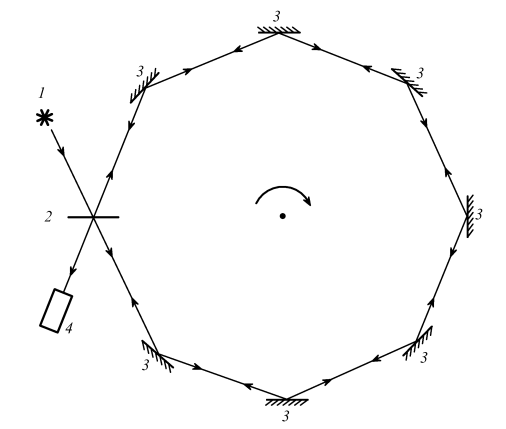
\includegraphics[width=\linewidth]{circle_interf}}
		\caption{
			Кольцевой интерферометр: \textbf{1} -- источник; \textbf{2} -- полупрозрачное зеркало; \textbf{3} -- зеркала; \textbf{4} -- приемник. Стрелкой указано направление вращения интерферометра.
		}
		\label{pic1}
	\end{wrapfigure}
	Пусть свет или некоторая волна произвольной природы	движется по окружности (рис. \ref{pic1}), что имеет место в обычном кольцевом интерферометре в случае, когда число расположенных по окружности зеркал или призм полного внутреннего отражения стремится к бесконечности.
	
	Приведем вывод на основе релятивистского закона сложения скоростей. Для произвольного типа волн, распространяющихся в произвольной среде с фазовой скоростью $v_\text{ф}^\pm$. Запишем выражения для длины пути $l^\pm$ в лабораторной (неподвижной) системе отсчета $K$, где специальная теория относительности заведомо справедлива (знак плюс соответствует волне, направление которой совпадает с направлением вращения):
	\newpage
	\begin{equation}
	\label{eq1}
	l^\pm = 2 \pi R \pm R \Omega t^\pm
	\end{equation}
	\begin{equation}
	\label{eq2}
		v_\text{ф}^\pm = \cfrac{v_\text{ф} \pm R \Omega}{1 \pm v_\text{ф} R \Omega^2 / c^2}
	\end{equation}
	Здесь $R$ -- радиус кольца, $\Omega$ -- угловая скорость вращения, $c$ -- скорость света в вакууме, $t^\pm = l^\pm / v_\text{ф}^\pm$ -- времена, затрачиваемые встречными волнами на обход кольца.
	
	Проведем рассмотрение эффекта Саньяка для случая, когда в кольцевом интерферометре распространяются два встречных импульса той или иной природы: при этом скоростями встречных импульсов являются их групповые скорости, которые могут быть получены путем релятивистского сложения их групповой скорости с линейной $R \Omega$ (с учетом знака).
	
	Для электромагнитных волн при отсутствии оптической среды фазовая и групповая скорости света совпадают и можно производить вычисления разности времен для групповых скоростей, а результаты расчета использовать для вычисления результата интерференции встречных волн. Однако в самом общем случае (а тем более для волн произвольной природы) для вычисления результатов интерференции встречных волн следует производить все промежуточные вычисления для фазовых скоростей. Мы ограничимся случаем электромагнитных волн. С более подробным выводом можно ознакомиться в \cite{Malykin:2000}.
	
	В четырехмерном пространстве Минковского выражение для фазы волны имеет вид:
	$$
	(\vec{k} \vec{r}) \pm \omega t = \phi = i n v
	$$
	Здесь $\vec{k} = \vec{x^0} k_x + \vec{y^0} k_y + \vec{z^0} k_z$ -- вектор, образованный волновыми числами $k_x$, $k_y$, $k_z$; $\vec{r} = \vec{x^0} x + \vec{y^0} y + \vec{z^0} z$; $k_i = 2 \pi n_i / \lambda$; $\omega$ -- круговая частота волны; $n_i$ -- коэффициент преломления вдоль $i$-го направления, $i=x,y,z$, $\vec{x^0}, \vec{y^0}, \vec{z^0}$ -- ортогональные единичные векторы; $\lambda$ -- длина волны. Фаза как скалярная величина инвариантна относительно преобразований Лоренца. При этом $\Delta \vec{r}/\Delta t = v_\text{гр}$ -- групповая скорость волны, $\omega / k = v_\text{ф}$ -- фазовая скорость волны, $k = \sqrt{k_x^2 + k_y^2 + k_z^2}$. 
	
	Определим величину фазовой скорости каждой из встречных волн как линейную скорость перемещения точки фиксированной фазы данной волны вдоль кольца. Согласно (\ref{eq1}), (\ref{eq2}) время для двух направлений $t^\pm$ будет:
	\begin{equation}
	\label{eq3}
		t^\pm = \cfrac{2 \pi R (1 \pm v_\text{ф} R \Omega/c^2)}{v_\text{ф} (1 - R^2 \Omega^2 / c^2)}
	\end{equation}
	Разность времен распространения для встречных волн составит:
	\begin{equation}
	\label{eq4}
	\Delta t = t^+ - t^- = \cfrac{4 \pi R^2 \Omega}{c^2 (1 - R^2 \Omega^2 / c^2)}
	\end{equation}
	Таким образом, разность времен, затрачиваемых встречными волнами на прохождение кольца, не зависит от фазовой скорости волн. Следовательно, разность времен, обусловленная эффектом Саньяка, не зависит от того, заполнен кольцевой интерферометр оптической средой или нет.
	
	Из выражения (\ref{eq4}) следует также, что волны, создающие интерференционную картину на делительном зеркале, т.е. пришедшие на него после обхода кольца одновременно, на входе кольца выходят из делительного зеркала в различные времена с разницей $\Delta t$. Поскольку здесь мы рассматриваем монохроматические гармонические колебания, то это никоим образом не влияет на видность интерференционной картины. Однако если в кольцевом интерферометре используются колебания со спектром конечной ширины, то при превышении величиной $\Delta t$ времени когерентности этих колебаний видность может существенно уменьшиться.
	
	Для вычисления разности фаз встречных волн целесообразно перейти в сопровождающую вращение кольцевого интерферометра систему отсчета $K'$. В соответствии с преобразованиями Лоренца разность времен распространения в это системе $K'$ составит:
	\begin{equation}
	\label{eq5}
	\Delta t' = \Delta t \sqrt{\left(1 - \cfrac{R^2 \Omega^2}{c^2}\right)} = \cfrac{4 \pi R^2 \Omega}{c^2 \sqrt{1 - R^2 \Omega^2 / c^2}}
	\end{equation}
	
	Разность фаз встречных волн на выходе кольца, обусловленная эффектом Саньяка, составит:
	\begin{equation}
	\label{eq6}
	\Phi_S = \omega \Delta t' = \cfrac{4 S \Omega \omega}{c^2 \sqrt{1 - R^2 \Omega^2 / c^2}} = \cfrac{8 \pi S \Omega \nu}{c^2 \sqrt{1 - R^2 \Omega^2 / c^2}}
	\end{equation}
	
	Здесь $\nu$ -- частота источника излучения в с.о. $K'$ в случае, если источник излучения расположен на расстоянии $R$ от центра вращения, т.е. непосредственно на кольце; $\omega = 2 \pi \nu$ -- круговая частота источника; $S = \pi R^2$ -- площадь кольца.
	
	Из выражения (\ref{eq6}) следуют два \textit{важных} вывода:
	\begin{enumerate}
		\item Величина разности фаз встречных волн не зависит от фазовой скорости волны, а зависит от частоты волны $\nu$. В частности, в оптическом диапазоне, где $v_\text{ф} = c / n$, она не зависит ни от коэффициента преломления $n$ оптической среды, заполняющей интерферометр, ни от дисперсии коэффициента преломления $\frac{dn}{d\lambda}$, причем вне зависимости от соотношения $R \Omega / c$.
		\item В выражении (\ref{eq2}) мы использовали релятивистский закон сложения фазовой скорости $v_\text{ф}$ и скорости вращения кольца $R \Omega$. Это соответствует тому, что эффект Саньяка является эффектом СТО. При этом использование галилеевского закона сложения скоростей при рассмотрении эффекта Саньяка, приводит к ошибочному результату, заключающемуся в отрицании существования данного эффекта.
		
	Тем не менее, вопрос о влиянии величины	коэффициента преломления среды и его дисперсии на величину эффекта Саньяка до сих пор обсуждается.
	\end{enumerate}
	
	\section{Проявление эффекта Саньяка в кольцевом интерферометре}
	Эффект Саньяка в чистом виде реализуется исключительно в ситуации, когда интерферометр и среда вращаются как единое целое. Для этого случая выражение (\ref{eq6}) примет вид:
	\begin{equation}
	\label{eq7}
	\Phi_S = \cfrac{8 \pi S \Omega}{\lambda c \sqrt{1 - R^2 \Omega^2 / c^2}}
	\end{equation}
	С другой стороны, в кольцевом интерферометре $\Phi_S = 2 \pi \Delta z$. Разность частот кольцевого \underline{лазера} $\Delta \nu$ обратна пропорциональна величине коэффициента преломления $n$ \cite{litlink5}; $\Omega = \const$.
	\begin{equation}
	\label{eq8}
	\Delta z = \cfrac{4 S \Omega n^2 (1- \alpha)}{\lambda c} = \cfrac{4 S \Omega}{\lambda c}, \tab \Delta \nu = \cfrac{4 S \Omega}{\lambda L n}
	\end{equation}
	
	Здесь $\alpha = 1 - 1/n^2$ называется коэффициентом увеличения Френеля, $S$ -- площадь кольцевого интерферометра, $\lambda$ -- длина волны света в вакууме.
	
	\section{Лазерный гироскоп}
	\begin{wrapfigure}{r}{0.5\linewidth}
		\centering{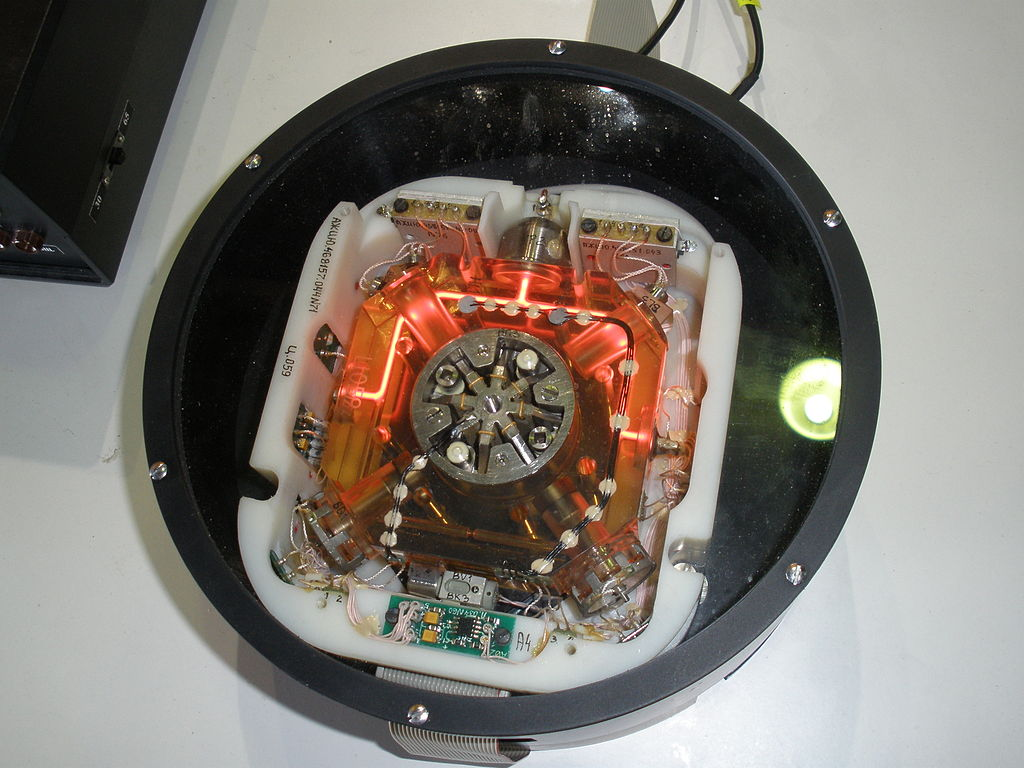
\includegraphics[width=\linewidth]{laser_gyro}}
		\caption{
			Кольцевой лазерный гироскоп производства украинского завода "Арсенал". Резонатор имеет форму квадрата. В его центре расположен виброподвес.
		}
		\label{pic2}
		\vspace{-30pt}
	\end{wrapfigure}
	\textit{ По материалам \href{https://ru.wikipedia.org/wiki/\%D0\%9B\%D0\%B0\%D0\%B7\%D0\%B5\%D1\%80\%D0\%BD\%D1\%8B\%D0\%B9\_\%D0\%B3\%D0\%B8\%D1\%80\%D0\%BE\%D1\%81\%D0\%BA\%D0\%BE\%D0\%BF}{Википедии}}
	
	\textbf{Лазерный гироскоп} -- оптический прибор для измерения угловой скорости, использующий эффект Саньяка. Обычно применяется в системах инерциальной навигации (навигации, не требующей внешних ориентиров).
	
	\subsection{Принцип работы}
	Прибор сам по себе является лазером и состоит из активной среды и резонатора, при работе происходит генерация излучения в двух направлениях. Работа лазерного гироскопа основана на уже описанном эффекте Саньяка, два луча генерируются в резонаторе лазерного гироскопа и, если прибор вращается, то происходит генерация волн разной частоты для разных направлений из-за различных эффективных длин резонатора для разных направлений обхода (вследствие вращения). Описать разность частот в гироскопе, вызванную вращением, можно с помощью полученной выше формулы (\ref{eq6}): $\Delta \nu = \cfrac{4 S \Omega}{L \lambda}$, где $S$ -- площадь, охватываемая лучом;  $L$ -- периметр резонатора, $\Omega$  -- угловая скорость вращения гироскопа, $\lambda$  -- длина волны.
	
	Резонатор лазерного гироскопа может быть достаточно сложным, но обычно это - кольцевой резонатор с тремя или четырьмя зеркалами.
	
	В лазерном гироскопе создаётся и поддерживается стоячая волна, а её узлы и пучности в идеальном случае связаны с инерциальной системой отсчёта. Таким образом, положение узлов и пучностей не меняется если гироскоп не вращается (в плоскости кольцевого контура) относительно инерциальной системы отсчёта, а при повороте резонатора (корпуса гироскопа) фотоприёмники измеряют угол поворота, считая пробегающие по ним интерференционные полосы.
	
	Чувствительность лазерного гироскопа пропорциональна площади поверхности, ограниченной лучами лазера.
	
	\subsection{Применение в исследованиях}
	Помимо навигации лазерный гироскоп можно применять для фундаментальных исследований или измерения колебаний земной коры (землетрясения). Для этих целей используются большие гироскопы, с периметром в несколько метров.
	
	Самый точный в мире лазерный гироскоп построен в геодезической обсерватории Веттцелль Мюнхенского технического университета. Он предназначен для фиксации тончайшего изменения смещения земной оси при вращении. Точность прибора такова, что он может улавливать биения земной оси в доли угловых минут.
	
	% Библиография
	\bibliography{references}
	\bibliographystyle{ieeetr}
	
\end{document}